%%%%%%%%%%%%%%%%%%%%%%%%%%%%%%%%%%%%%%%%%
% Structured General Purpose Assignment
% LaTeX Template
%
% This template has been downloaded from:
% http://www.latextemplates.com
%
% Original author:
% Ted Pavlic (http://www.tedpavlic.com)
%
% Note:
% The \lipsum[#] commands throughout this template generate dummy text
% to fill the template out. These commands should all be removed when 
% writing assignment content.
%
%%%%%%%%%%%%%%%%%%%%%%%%%%%%%%%%%%%%%%%%%


%----------------------------------------------------------------------------------------
%	PACKAGES AND OTHER DOCUMENT CONFIGURATIONS
%----------------------------------------------------------------------------------------

\documentclass{article}

%\usepackage{currfile}
\usepackage{fancyhdr} % Required for custom headers
\usepackage{lastpage} % Required to determine the last page for the footer
\usepackage{extramarks} % Required for headers and footers
\usepackage{graphicx} % Required to insert images
\usepackage{lipsum} % Used for inserting dummy 'Lorem ipsum' text into the template
\usepackage{outlines}
\usepackage{wrapfig}
\usepackage[dutch,]{babel}
\selectlanguage{dutch}

\usepackage{xcolor}
\usepackage{listings}	% om SQL code toe te voegen aan document

% Margins
\topmargin=-0.45in
\evensidemargin=0in
\oddsidemargin=0in
%\textwidth=6.5in
\textwidth=6.8in
\textheight=9.0in
\headsep=0.25in 

\linespread{1.1} % Line spacing

% Set up the header and footer
\pagestyle{fancy}
\lhead{\hmwkAuthorName} % Top left header
%\chead{\hmwkClass\ \small{(\textit{\hmwkClassInstructor})}} 
\chead{\hmwkClass} 
\rhead{\hmwkTitle} 
\lfoot{\LaTeX: \small{\input{filename.txt}}} % Bottom left footer
%\lfoot{\LaTeX: {/home/jan/CVOTSM/A7\_IT-organisatie/ITIL/}\currfilepath} % Bottom left footer
\cfoot{} % Bottom center footer
\rfoot{Pagina\ \thepage\ van\ \pageref{LastPage}} % Bottom right footer
\renewcommand\headrulewidth{0.4pt} % Size of the header rule
\renewcommand\footrulewidth{0.4pt} % Size of the footer rule

\setlength\parindent{0pt} % Removes all indentation from paragraphs


%\setlength{\parskip}{\baselineskip}%
%\setlength{\parindent}{12pt}%

%----------------------------------------------------------------------------------------
%	DOCUMENT STRUCTURE COMMANDS
%	Skip this unless you know what you're doing
%----------------------------------------------------------------------------------------

% Header and footer for when a page split occurs within a problem environment
\newcommand{\enterProblemHeader}[1]{
\nobreak\extramarks{#1}{#1 continued on next page\ldots}\nobreak
\nobreak\extramarks{#1 (continued)}{#1 continued on next page\ldots}\nobreak
}

% Header and footer for when a page split occurs between problem environments
\newcommand{\exitProblemHeader}[1]{
\nobreak\extramarks{#1 (continued)}{#1 continued on next page\ldots}\nobreak
\nobreak\extramarks{#1}{}\nobreak
}

\setcounter{secnumdepth}{0} % Removes default section numbers
\newcounter{homeworkProblemCounter} % Creates a counter to keep track of the number of problems

\newcommand{\homeworkProblemName}{}
\newenvironment{homeworkProblem}[1][Problem \arabic{homeworkProblemCounter}]{ % Makes a new environment called homeworkProblem which takes 1 argument (custom name) but the default is "Problem #"
\stepcounter{homeworkProblemCounter} % Increase counter for number of problems
\renewcommand{\homeworkProblemName}{#1} % Assign \homeworkProblemName the name of the problem
\section{\homeworkProblemName} % Make a section in the document with the custom problem count
\enterProblemHeader{\homeworkProblemName} % Header and footer within the environment
}{
\exitProblemHeader{\homeworkProblemName} % Header and footer after the environment
}

\newcommand{\problemAnswer}[1]{ % Defines the problem answer command with the content as the only argument
\noindent\framebox[\columnwidth][c]{\begin{minipage}{0.98\columnwidth}#1\end{minipage}} % Makes the box around the problem answer and puts the content inside
}

\newcommand{\homeworkSectionName}{}
\newenvironment{homeworkSection}[1]{ % New environment for sections within homework problems, takes 1 argument - the name of the section
\renewcommand{\homeworkSectionName}{#1} % Assign \homeworkSectionName to the name of the section from the environment argument
\subsection{\homeworkSectionName} % Make a subsection with the custom name of the subsection
\enterProblemHeader{\homeworkProblemName\ [\homeworkSectionName]} % Header and footer within the environment
}{
\enterProblemHeader{\homeworkProblemName} % Header and footer after the environment
}
   
%----------------------------------------------------------------------------------------
%	NAME AND CLASS SECTION
%----------------------------------------------------------------------------------------

\newcommand{\hmwkTitle}{4. Klassendiagram} % Assignment title
%\newcommand{\hmwkDueDate}{Monday,\ January\ 1,\ 2012} % Due date
\newcommand{\hmwkDueDate}{} % Due date
\newcommand{\hmwkClass}{Projectwerk} % Course/class
%\newcommand{\hmwkClassTime}{10:30am} % Class/lecture time
\newcommand{\hmwkClassTime}{} % Class/lecture time
\newcommand{\hmwkClassInstructor}{} % Teacher/lecturer
\newcommand{\hmwkAuthorName}{Wagemakers Jan} % Your name

%----------------------------------------------------------------------------------------
%	TITLE PAGE
%----------------------------------------------------------------------------------------

\title{
\vspace{2in}
\textmd{\textbf{\hmwkClass}}\\
\textmd{\textbf{\hmwkTitle}}\\
%\normalsize\vspace{0.1in}\small{In\ te\ dienen\ voor\ \hmwkDueDate}\\
%\vspace{0.1in}{\textit{Leerkracht: \hmwkClassInstructor\ \hmwkClassTime}}
\vspace{3in}
}

\author{\textbf{\hmwkAuthorName}}
\date{\today} % Insert date here if you want it to appear below your name

%----------------------------------------------------------------------------------------

\begin{document}

\maketitle

%----------------------------------------------------------------------------------------
%	TABLE OF CONTENTS
%----------------------------------------------------------------------------------------

%\setcounter{tocdepth}{1} % Uncomment this line if you don't want subsections listed in the ToC

%\newpage
%\tableofcontents
\newpage

%%% Opdracht

%\begin{homeworkProblem}[\arabic{homeworkProblemCounter} : Omschrijving opdracht]
%\begin{homeworkProblem}[Schematisch overzicht gegevens]
%	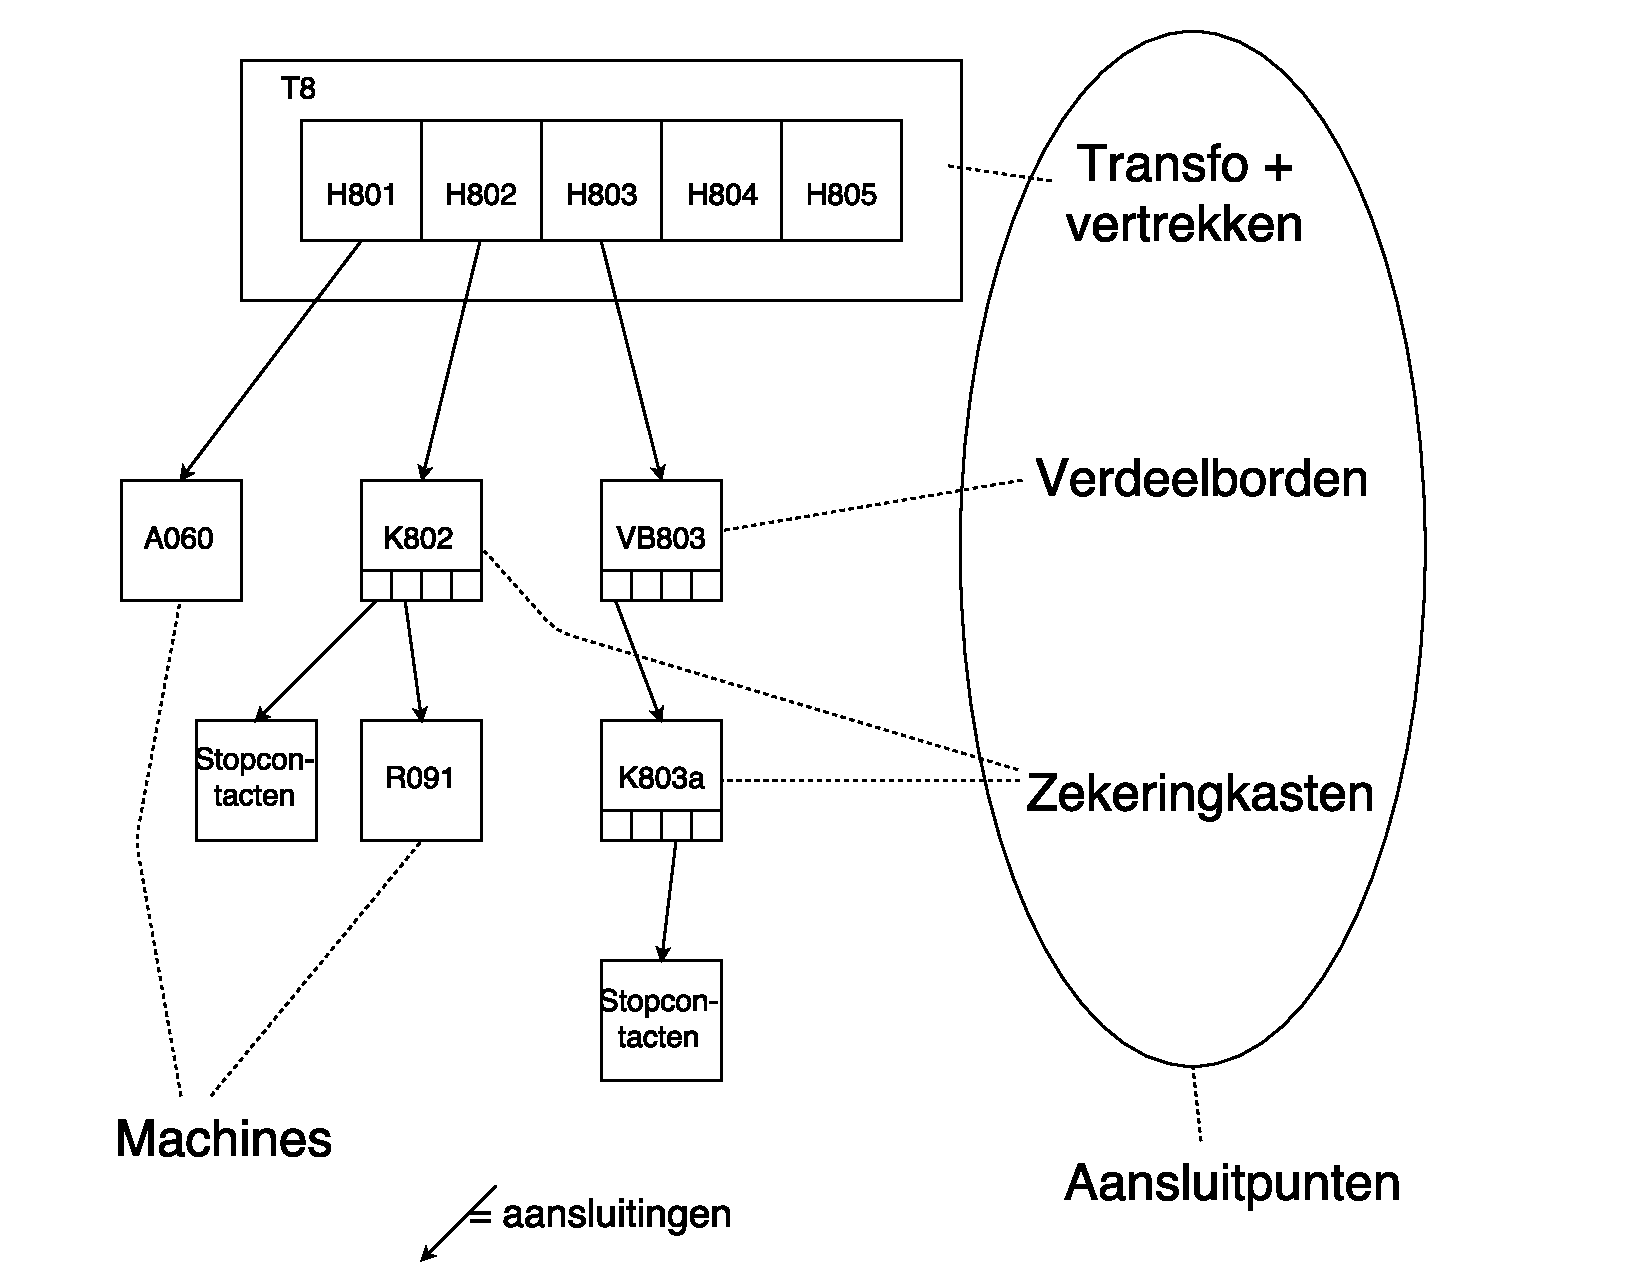
\includegraphics[width=1.2\textwidth]{pictures/Aansluitpunten.ps}
%\end{homeworkProblem}
%\newpage
\begin{homeworkProblem}[Klassendiagram]

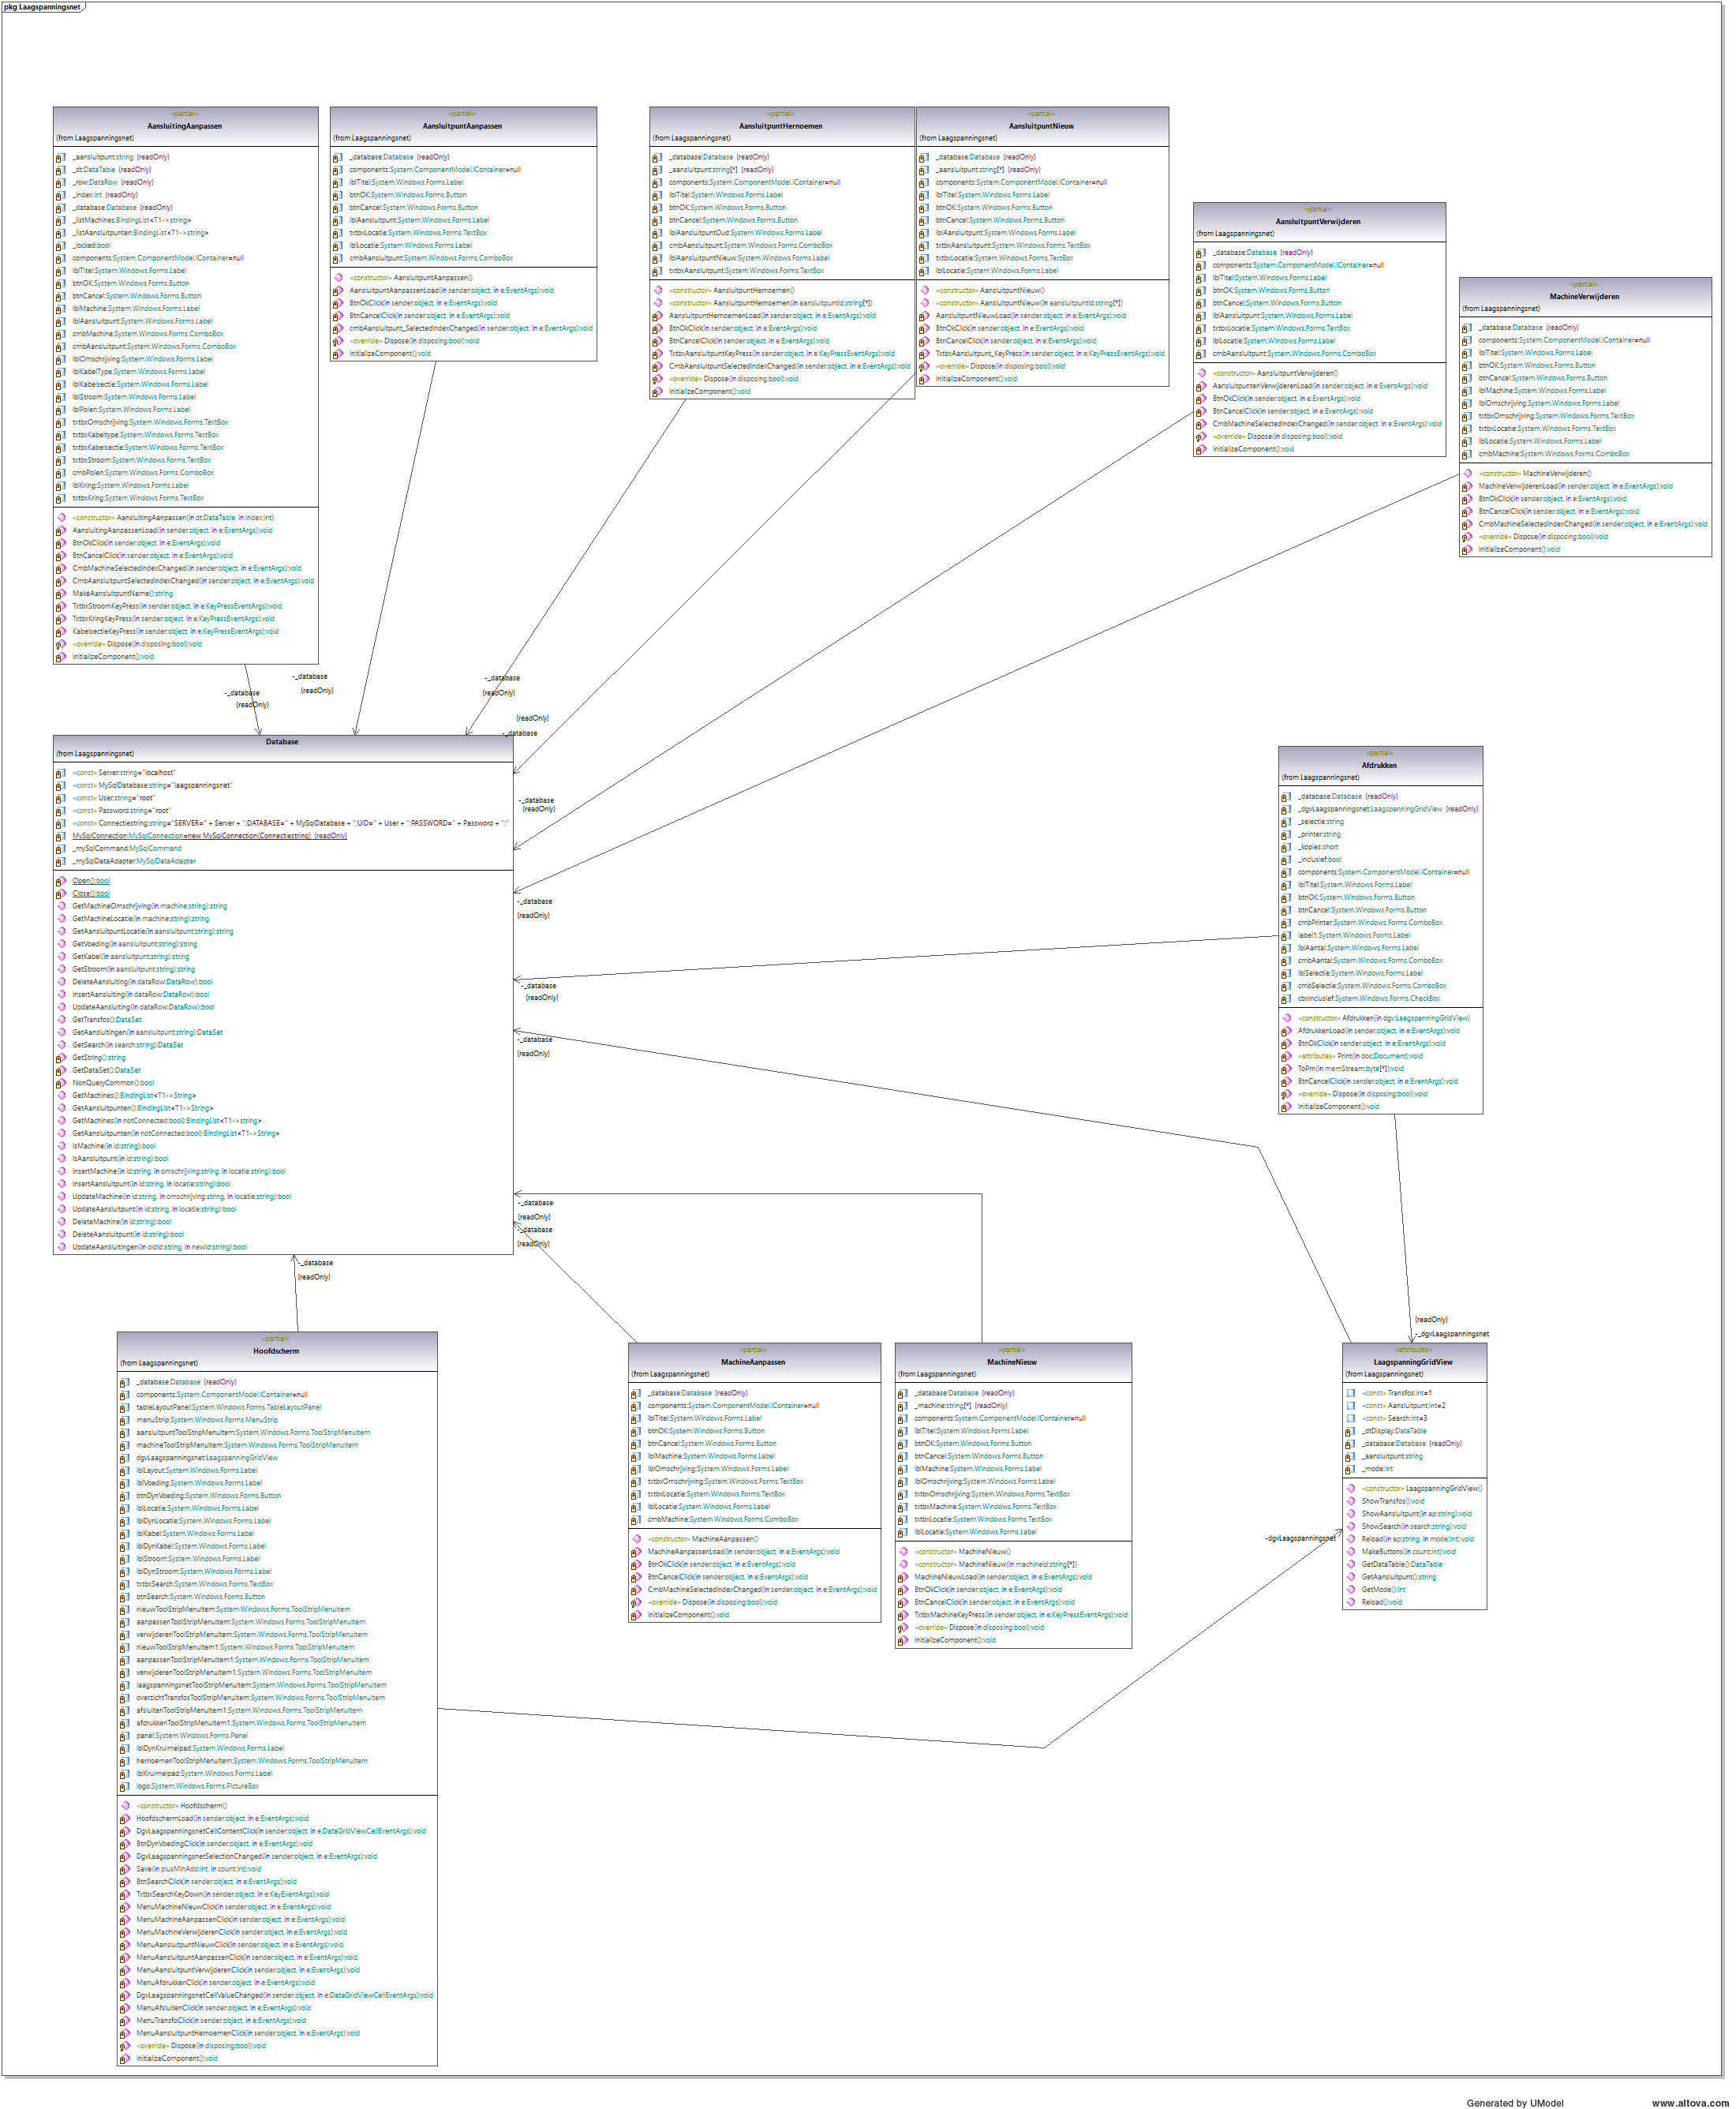
\includegraphics[width=1.05\textwidth]{/home/jan/MEGA/2017-2018/ProjectWerk/source/repos/Laagspanningsnet/Laagspanningsnet.png}
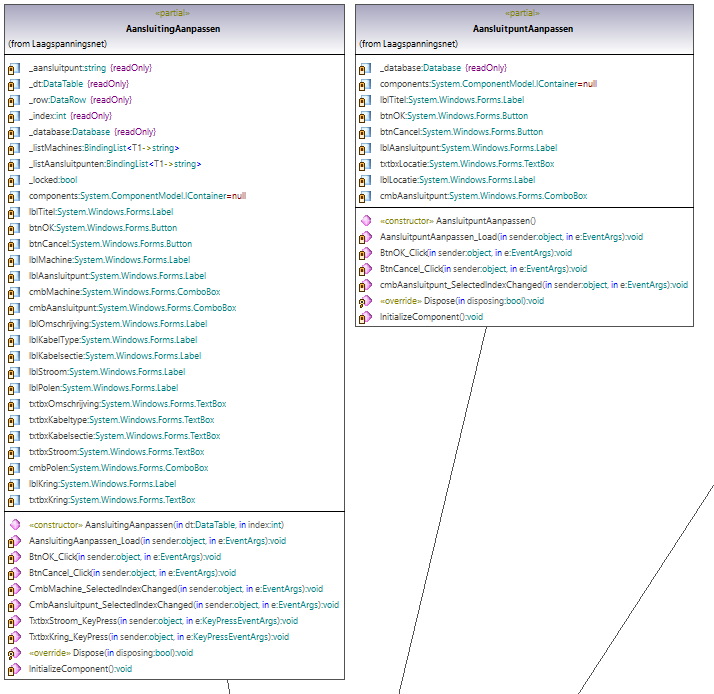
\includegraphics[width=1.05\textwidth]{/home/jan/MEGA/2017-2018/ProjectWerk/source/repos/Laagspanningsnet/LaagspanningsnetP1.png}
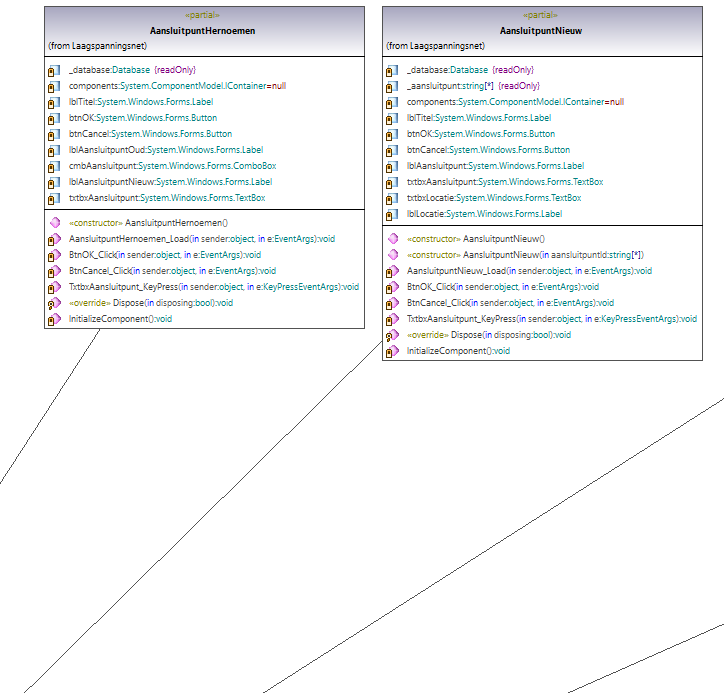
\includegraphics[width=1.05\textwidth]{/home/jan/MEGA/2017-2018/ProjectWerk/source/repos/Laagspanningsnet/LaagspanningsnetP2.png}
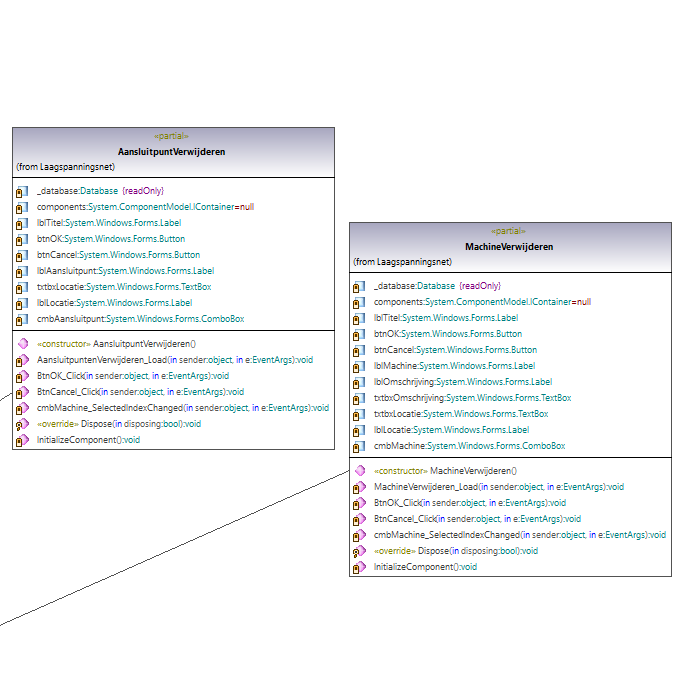
\includegraphics[width=1.05\textwidth]{/home/jan/MEGA/2017-2018/ProjectWerk/source/repos/Laagspanningsnet/LaagspanningsnetP3.png}
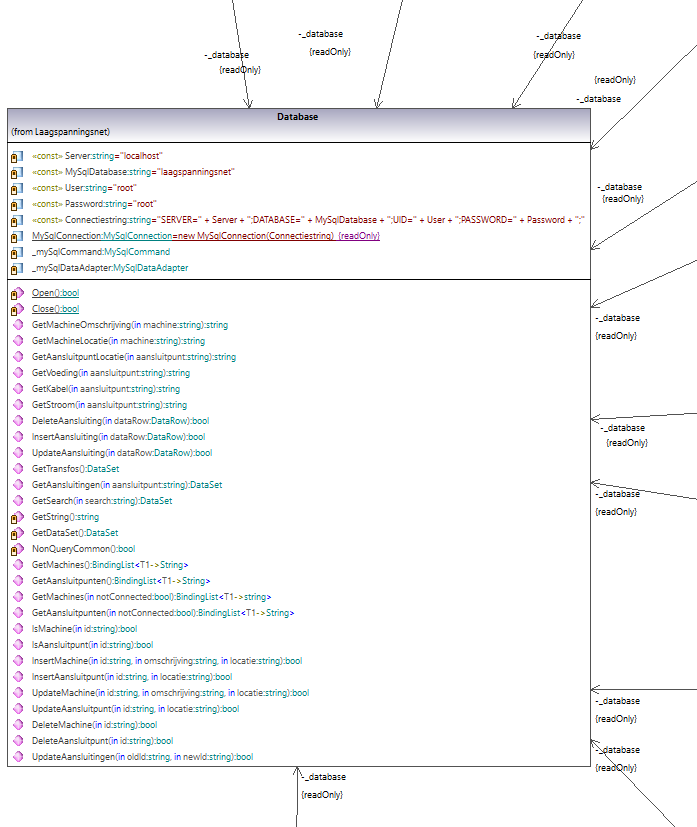
\includegraphics[width=1.05\textwidth]{/home/jan/MEGA/2017-2018/ProjectWerk/source/repos/Laagspanningsnet/LaagspanningsnetP4.png}
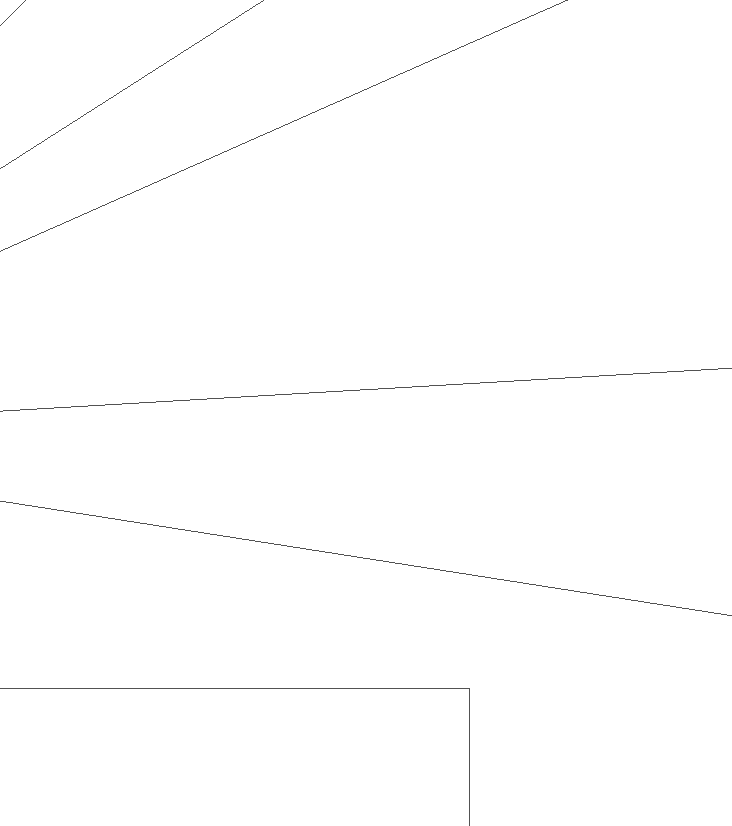
\includegraphics[width=1.05\textwidth]{/home/jan/MEGA/2017-2018/ProjectWerk/source/repos/Laagspanningsnet/LaagspanningsnetP5.png}
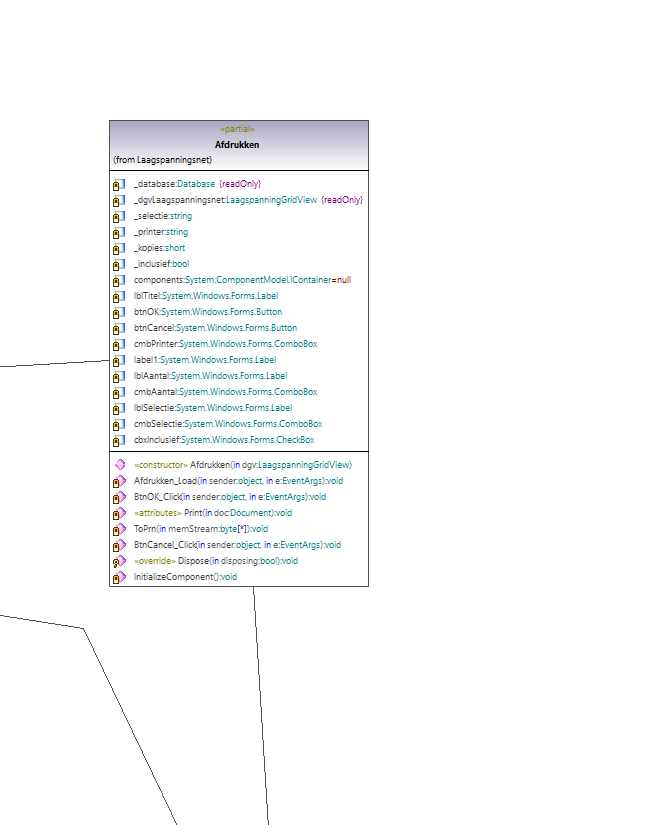
\includegraphics[width=1.05\textwidth]{/home/jan/MEGA/2017-2018/ProjectWerk/source/repos/Laagspanningsnet/LaagspanningsnetP6.png}
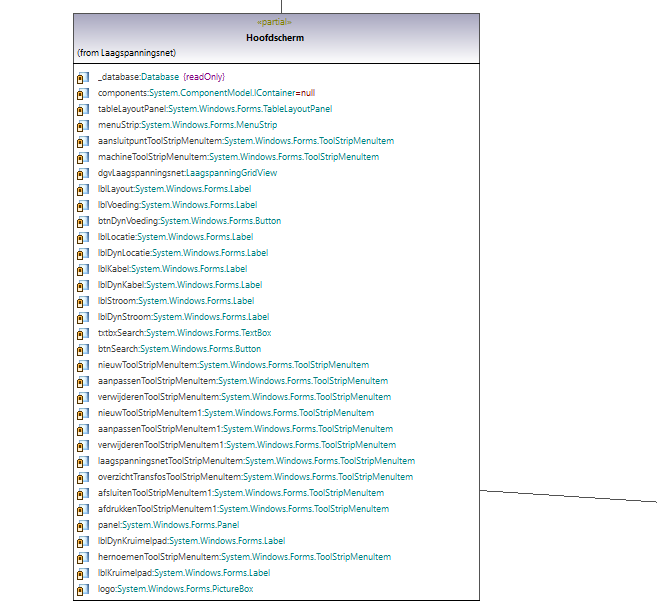
\includegraphics[width=1.05\textwidth]{/home/jan/MEGA/2017-2018/ProjectWerk/source/repos/Laagspanningsnet/LaagspanningsnetP7.png}
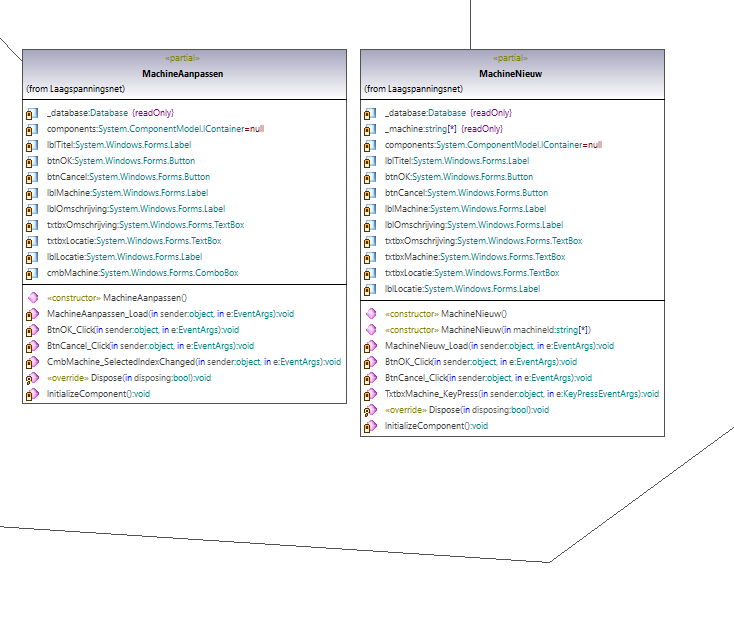
\includegraphics[width=1.05\textwidth]{/home/jan/MEGA/2017-2018/ProjectWerk/source/repos/Laagspanningsnet/LaagspanningsnetP8.png}
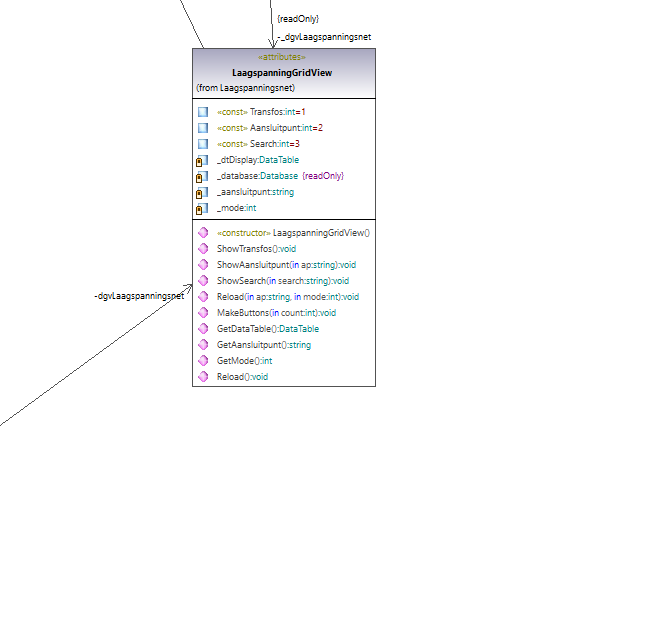
\includegraphics[width=1.05\textwidth]{/home/jan/MEGA/2017-2018/ProjectWerk/source/repos/Laagspanningsnet/LaagspanningsnetP9.png}
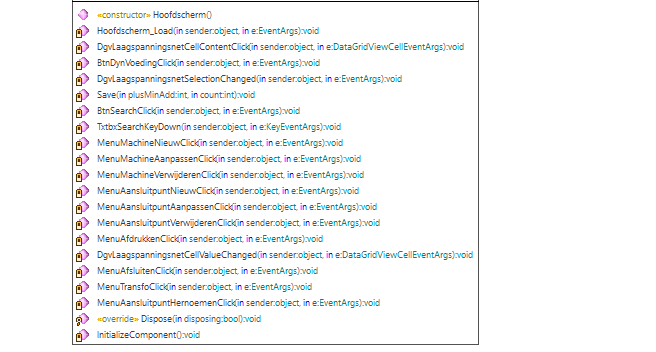
\includegraphics[width=1.05\textwidth]{/home/jan/MEGA/2017-2018/ProjectWerk/source/repos/Laagspanningsnet/LaagspanningsnetP10.png}


\end{homeworkProblem}
\end{document}


\begin{homeworkProblem}[Database]
\begin{itemize}
\item\textbf{Doel} : alle communciatie met de database verloopt via deze klasse.
\item\textbf{Atributen} 
	\begin{itemize}
        \item \textcolor{blue}{\textbf{$-$string Server}}
        \item \textcolor{blue}{\textbf{$-$string MySqlDatabase}}
        \item \textcolor{blue}{\textbf{$-$string User}}
        \item \textcolor{blue}{\textbf{$-$string Password}}
        \item \textcolor{blue}{\textbf{$-$string Connectiestring}}
        \item \textcolor{blue}{\textbf{$-$MySqlConnection \underline{MySqlConnection}}}
	\item \textcolor{blue}{\textbf{$-$MySqlDataAdapter \_mySqlDataAdapter}}
	\item \textcolor{blue}{\textbf{$-$MySqlCommand \_mysqlCommand}}
\_mySqlDataAdapter}}
	\end{itemize}
\item\textbf{Constructor}
        \begin{itemize}
                \item\textcolor{blue}{\textbf{$+$Database()}}
        \end{itemize}
\item\textbf{Methodes}
	\begin{itemize}
	\item \textcolor{blue}{\textbf{$-$\underline{Open}():bool}}
		\begin{itemize}
			\item \textbf{Doel} : openen van een connectie met de database.
			\item \textbf{Parameters} : geen.
			\item \textbf{Return} : bool 
				\begin{itemize}
					\item false = mislukt 
					\item true = connectie is geopend
				\end{itemize}
		\end{itemize}
        \item \textcolor{blue}{\textbf{$-$\underline{Close}():bool}}
        	\begin{itemize}
			\item \textbf{Doel} : sluiten van de connectie met de database.
			\item \textbf{Parameters} : geen.
			\item \textbf{Return} : bool 
				\begin{itemize}
					\item false = mislukt 
					\item true = connectie is gesloten
				\end{itemize}
		\end{itemize}
	\item \textcolor{blue}{\textbf{$+$GetMachineOmschrijving(string machine):}}
                \begin{itemize}
                        \item \textbf{Doel} : sluiten van de connectie met de database.
                        \item \textbf{Parameters} : geen.
                        \item \textbf{Return} : bool
                                \begin{itemize}
                                        \item false = mislukt
                                        \item true = connectie is gesloten
                                \end{itemize}
                \end{itemize}









	\item\textcolor{blue}{\textbf{$+$GetTransfos():DataSet}}
        	\begin{itemize}
			\item \textbf{Doel} : ophalen van alle transformatoren die op het bedrijf aanwezig zijn.
			\item \textbf{Parameters} : geen.
			\item \textbf{Return} : DataSet met gegevens van alle transformatoren
		\end{itemize}
	\item  \textcolor{blue}{\textbf{$+$GetAansluitingen(String aansluitpunt):DataSet}}
		\begin{itemize}
                        \item \textbf{Doel} : opvragen van alle aansluitingen die behoren tot een bepaalde aansluitpunt
                        \item \textbf{Parameters} : String aansluitpunt
                        \item \textbf{Return} : DataSet met gegevens van alle aansluitingen van een aansluitpunt
                \end{itemize}
	\item  \textcolor{blue}{\textbf{$+$GetSearch(String search):DataSet}}
		\begin{itemize}
                        \item \textbf{Doel} : ophalen van zoekresultaten
                        \item \textbf{Parameters} : String search, waarbij search de zoekterm is
                        \item \textbf{Return} : DataSet met alle zoekresultaten
                \end{itemize}
	\item  \textcolor{blue}{\textbf{$+$GetMachineOmschrijving(String machine):String}}
		\begin{itemize}
                        \item \textbf{Doel} : opvragen van de omschrijving van een bepaalde machine
                        \item \textbf{Parameters} : String machine
                        \item \textbf{Return} : String met de omschrijving
                \end{itemize}
        \item \textcolor{blue}{\textbf{ $+$GetMachineLocatie(String machine):String}}
		\begin{itemize}
                        \item \textbf{Doel} : opvragen van de locatie van een bepaalde machine
                        \item \textbf{Parameters} : String machine
                        \item \textbf{Return} : String met de locatie
                \end{itemize}
	\item \textcolor{blue}{\textbf{ $+$GetAansluitpuntLocatie(String aansluitpunt):String}}
		\begin{itemize}
                        \item \textbf{Doel} : opvragen van de locatie van een bepaalde aansluitpunt
                        \item \textbf{Parameters} : String aansluitpunt
                        \item \textbf{Return} : String met de locatie
                \end{itemize}
	\item  \textcolor{blue}{\textbf{$+$GetVoeding(String aansluitpunt):String}}
		\begin{itemize}
                        \item \textbf{Doel} : opvragen van de voeding van een bepaald aansluitpunt
                        \item \textbf{Parameters} : String aansluitpunt
                        \item \textbf{Return} : String met de voeding, = "-" als er geen voeding is gevonden
                \end{itemize}
	\item  \textcolor{blue}{\textbf{$+$GetKabel(String aansluitpunt):String}}
		\begin{itemize}
                        \item \textbf{Doel} : opvragen van de voedingskbal van een bepaald aansluitpunt
                        \item \textbf{Parameters} : String aansluitpunt
                        \item \textbf{Return} : String met de voedingskabel, = "-" als er geen voedingskabel is gevonden
                \end{itemize}
	\item \textcolor{blue}{ \textbf{$+$GetStroom(String aansluitpunt):String}}
		\begin{itemize}
                       \item \textbf{Doel} : opvragen van de stroomtoevoer (voeding) van een bepaald aansluitpunt
                        \item \textbf{Parameters} : String aansluitpunt
                        \item \textbf{Return} : String met de stroom, = "-" als er geen voeding is gevonden
                \end{itemize}
	\item  \textcolor{blue}{\textbf{$+$SetAansluitingen(DataSet dsDatabase):bool}}
		\begin{itemize}
                        \item \textbf{Doel} : data van alle aansluitingen van een aansluitpunt opslaan in de database
                        \item \textbf{Parameters} : DataSet dsDatabase met alle aansluitingen van een aansluitpunt
                        \item \textbf{Return} : bool
				\begin{itemize}
                                        \item false = mislukt
                                        \item true = connectie is gesloten
                                \end{itemize}
                \end{itemize}
	\item \textcolor{cyan}{\textbf{$-$GetString(String query):String}}
		\begin{itemize}
			\item \textbf{Doel} : ophalen van een string uit de database. Dit is een private gemeenschappelijke routine die door andere methodes gebruikt wordt.
			\item \textbf{Parameters} : String query met de query op de MySql-server moet worden uitgevoerd.
			\item \textbf{Return} : String met het resultaat.
		\end{itemize}
	\item \textcolor{cyan}{\textbf{$-$GetDataSet(String query):DataSet}}
		\begin{itemize}
			\item \textbf{Doel} : ophalen van een DataSet uit de database. Dit is een private gemeenschappelijke routine die door andere methodes gebruikt wordt.
			\item \textbf{Parameters} : String query met de query op de MySql-server moet worden uitgevoerd.
                        \item \textbf{Return} : DataSet met het resultaat.
		\end{itemize}
	\item \textcolor{cyan}{\textbf{$-$NonQueryCommon(String nonQuery):bool}}
		\begin{itemize}
			\item \textbf{Doel} : Gemeenschappelijke routine voor INSERT/UPDATE/DELETE die door andere methodes gebruikt wordt.
			\item \textbf{Parameters} : String nonQuery met het INSERT/UPDATE/DELETE SQL commando.
			\item \textbf{Return} : bool
                                \begin{itemize}
                                        \item false = mislukt
                                        \item true = connectie is gesloten
                                \end{itemize}
		\end{itemize}
	\item \textcolor{blue}{\textbf{$+$GetMachines():List$<$String$>$}}
		\begin{itemize}
			\item \textbf{Doel} : Lijst ophalen van alle machines die in de machine table aanwezig zijn.
			\item \textbf{Parameters} : geen.
			\item \textbf{Return} : List$<$String$>$ met een lijst van alle machines
      		\end{itemize} 
	\item \textcolor{blue}{\textbf{$+$GetMachines(bool notConnected):List$<$String$>$}}
		\begin{itemize}
                        \item \textbf{Doel} : Lijst ophalen van machines uit de machine table.
                        \item \textbf{Parameters} : bool notConnected
				\begin{itemize}
                                        \item false = alle machines uit de machine table ophalen (=\textbf{$+$GetMachines():List$<$String$>$})
                                        \item true = enkel niet aangesloten machines uit de machine table ophalen
                                \end{itemize}
                        \item \textbf{Return} : List$<$String$>$ met een lijst van de machines
                \end{itemize} 
        \item \textcolor{blue}{\textbf{$+$GetAansluitpunten():List$<$String$>$}}
                \begin{itemize}
                        \item \textbf{Doel} : Lijst ophalen van alle aansluitpunten die in de aansluitpunt table aanwezig zijn.
                        \item \textbf{Parameters} : geen.
                        \item \textbf{Return} : List$<$String$>$ met een lijst van alle aansluitpunten
                \end{itemize} 
	\item \textcolor{blue}{\textbf{$+$GetAansluitpunten(bool notConnected):List$<$String$>$}}
                \begin{itemize}
                        \item \textbf{Doel} : Lijst ophalen van aansluitpunten uit de aansluitpunt table.
                        \item \textbf{Parameters} : bool notConnected
                                \begin{itemize}
                                        \item false = alle aansluitpunten uit de aansluitpunt table ophalen (=\textbf{$+$GetAansluitpunten():List$<$String$>$})
                                        \item true = enkel niet aangesloten aansluitpunten uit de aansluitpunt table ophalen
                                \end{itemize}
                        \item \textbf{Return} : List$<$String$>$ met een lijst van de aansluitpunten
                \end{itemize} 
\end{itemize}
\end{itemize}
\end{homeworkProblem}

\begin{homeworkProblem}[Hoofdscherm : Form]
\begin{itemize}
\item\textbf{Doel} : Het hoofdscherm van het programma opbouwen. Deze klasse
communiceert met de \textbf{Database}-klasse om de nodige gegevens uit de
database op te halen. Andere vensters worden van uit deze klasse aangeroepen.
\item\textbf{Atributen}
        \begin{itemize}
	\item \textcolor{blue}{\textbf{$-$Database database}} : Alle communicatie met de database verloopt via de database klasse
        \item \textcolor{blue}{\textbf{$-$DataTable dtDisplay}} : Inhoud van deze DataTable wordt via een DataGridView op het scherm getoond
        \item \textcolor{blue}{\textbf{$-$bool unsaved}} : Staan er niet bewaarde gegevens op het scherm?
        \item \textcolor{blue}{\textbf{$-$string aansluitpunt}} : Het aansluitpunt dat momenteel wordt getoond
\end{itemize}
\item\textbf{Constructor}
        \begin{itemize}
                \item\textcolor{blue}{\textbf{$+$Hoofdscherm()}}
        \end{itemize}
\item\textbf{Methodes}
	\begin{itemize}
        \item  \textcolor{blue}{\textbf{$-$ShowTransfos()}}
		\begin{itemize}
                        \item \textbf{Doel} : Tonen van overzicht van alle transfos op het scherm
                        \item \textbf{Parameters} : geen.
                        \item \textbf{Return} : niets.
		\end{itemize}

	\item  \textcolor{blue}{\textbf{$-$ShowAansluitpunt(String aansluitpunt)}}
		\begin{itemize}
                        \item \textbf{Doel} : Tonen van alle aansluitingen van een bepaald aansluitpunt
                        \item \textbf{Parameters} : String aansluitpunt
                        \item \textbf{Return} : niets.
                \end{itemize}

	\item  \textcolor{blue}{\textbf{$-$ShowSearch(String search)}}
                \begin{itemize}
                        \item \textbf{Doel} : Tonen van de zoekresultaten
                        \item \textbf{Parameters} : String met de zoekterm
                        \item \textbf{Return} : niets.
                \end{itemize}

        \item  \textcolor{cyan}{\textbf{$-$ShowCommon(String word, int modus)}} 
		\begin{itemize}
                        \item \textbf{Doel} : Tijdens het programmeren is gebleken dat er veel code gemeenschappelijk is tussen \textbf{showTransfos},
				\textbf{showAansluitpunt}, \textbf{showSearch}, daarom is deze gemeenschappelijke routine aangemaakt.
                        \item \textbf{Parameters} : String zoekterm/aansluitpunt, int modus 1=Transfos, 2=Aansluitpunt, 3=Search
                        \item \textbf{Return} : niets.
                \end{itemize}
	\item \textcolor{blue}{\textbf{$-$DgvLaagspanningsnet\_CellContentClick(object sender, DataGridViewCellEventArgs e)}}
                \begin{itemize}
                        \item \textbf{Doel} : Actie ondernemen als er op een Cell van de DataGridView wordt geklikt
                        \item \textbf{Parameters} : object sender, DataGridViewCellEventArgs e
                        \item \textbf{Return} : niets.
                \end{itemize}
	\item  \textcolor{blue}{\textbf{$-$BtnDynVoeding\_Click(object sender, EventArgs e)}}
                \begin{itemize}
                        \item \textbf{Doel} : Actie ondernemen als er op de voedingsknop is geklikt
                        \item \textbf{Parameters} : object sender, EventArgs e
                        \item \textbf{Return} : niets.
                \end{itemize}
	\item  \textcolor{blue}{\textbf{$-$SetUnsaved(bool status)}}
                \begin{itemize}
                        \item \textbf{Doel} : Bijhouden of data reeds in de database is opgeslagen
                        \item \textbf{Parameters} : bool status
				\begin{itemize}
					\item false : database- en scherm-inhoud komen overeen
					\item true : niet alle gegevens zijn bewaard
				\end{itemize}
                        \item \textbf{Return} : niets.
                \end{itemize}
	\item  \textcolor{cyan}{\textbf{$-$DgvLaagspanningsnet\_SelectionChanged(object sender, EventArgs e)}}
                \begin{itemize}
                        \item \textbf{Doel} : Uitschakelen van blauwe selectiebalk in DataGridView\\ (zie ook: https://stackoverflow.com/questions/11330147/how-to-disable-the-ability-to-select-in-a-datagridview)
                        \item \textbf{Parameters} : object sender, EventArgs e
                        \item \textbf{Return} : niets.
                \end{itemize}
	\item  \textcolor{blue}{\textbf{$-$BtnSave\_Click(object sender, EventArgs e)}}
		\begin{itemize}
			\item \textbf{Doel} : Actie ondernemen als er op de save-knop wordt geklikt
			\item \textbf{Parameters} : object sender, EventArgs e
			\item \textbf{Return} : niets.
		\end{itemize}
       \item  \textcolor{blue}{\textbf{$-$BtnUndo\_Click(object sender, EventArgs e)}}
                \begin{itemize}
                        \item \textbf{Doel} : Actie ondernemen als er op de undo-knop wordt geklikt
                        \item \textbf{Parameters} : object sender, EventArgs e
                        \item \textbf{Return} : niets.
                \end{itemize}
	\item  \textcolor{blue}{\textbf{$-$BtnSearch\_Click(object sender, EventArgs e)}}
                \begin{itemize}
                        \item \textbf{Doel} : Actie ondernemen als er op de zoek-knop wordt geklikt
                        \item \textbf{Parameters} : object sender, EventArgs e
                        \item \textbf{Return} : niets.
                \end{itemize}
	\item \textcolor{cyan}{\textbf{$-$TxtbxSearch\_KeyDown(object sender, KeyEventArgs e)}}
		\begin{itemize}
                        \item \textbf{Doel} : Op Enter drukken in de search box = op zoekknop klikken.
                        \item \textbf{Parameters} : object sender, EventArgs e
                        \item \textbf{Return} : niets.
                \end{itemize}
	\item \textcolor{cyan}{\textbf{$-$MakeButtons(int index)}}
		\begin{itemize}
			\item \textbf{Doel} : Maak van row(index) van de DataGridView de knoppen aan voor +/-/A en aansluitpunt. Maak van de laatste row met enkel het $+$-teken alles grijs.
			\item \textbf{Parameters} : int index : index van de row
			\item \textbf{Return} : niets.
		\end{itemize}
	 \end{itemize}
\end{itemize}
\end{homeworkProblem}

\begin{homeworkProblem}[AansluitingAanpassen : Form]
\begin{itemize}
\item\textbf{Doel} : Het scherm tonen waarmee de inhoud van /'e/'en aansluiting aangepast kan worden. Deze klasse wordt aangeroepen door de klasse \textbf{Hoofdscherm}. Bij de aanroep worden als parameters de DataTable 
meegegeven van de aansluitingen die getoond worden en de index van de aansluiting die aangepast moet worden. De reden dat de volledige DataTable wordt doorgegeven is om te kunnen testen of de ingegeven aansluiting wel uniek is.
Verder communiceert deze klasse met de \textbf(Database)-klasse om de machine- en aansluitpunt-lijst e.d. op te halen. Deze klasse zal echter geen aanpassingen in de database maken. 
\item\textbf{Atributen}
        \begin{itemize}
		\item \textcolor{blue}{\textbf{$-$string aansluitpunt}} : Het aansluitpunt waarvan een aansluiting aangepast wordt.
	        \item \textcolor{blue}{\textbf{$-$Database database}} : Alle communicatie met de database verloopt via de database klasse
		\item \textcolor{blue}{\textbf{$-$DataRow row}} : De DataRow met de aansluiting die aangepast wordt.
		\item \textcolor{cyan}{\textbf{$-$DataTable dt}} : DataTable met alle aansluitingen van het aansluitpunt.
		\item \textcolor{cyan}{\textbf{$-$int index}} : index van de row.        
	\end{itemize}
\item\textbf{Constructor}
	\begin{itemize}
		\item \textcolor{cyan}{\textbf{$+$AansluitingAanpassen(DataTable dt, int index)}}
		\begin{itemize}
			\item\textbf{Parameters} : 
			\begin{itemize}
				\item DataTable dt : DataTable met alle aansluitingen van het aansluitpunt
				\item int index : index van de aan te passen row
			\end{itemize}
		\end{itemize}
	\end{itemize}
\item\textbf{Methodes}
        \begin{itemize}
	\item  \textcolor{blue}{\textbf{$-$BtnOK\_Click(object sender, EventArgs e)}}
                \begin{itemize}
                        \item \textbf{Doel} : Actie ondernemen als er op de OK-knop wordt geklikt
                        \item \textbf{Parameters} : object sender, EventArgs e
                        \item \textbf{Return} : niets.
                \end{itemize}        
	\item  \textcolor{blue}{\textbf{$-$BtnCancel\_Click(object sender, EventArgs e)}}
                \begin{itemize}
                        \item \textbf{Doel} : Actie ondernemen als er op de Cancel-knop wordt geklikt, dit zal uiteindelijk het venster sluiten
                        \item \textbf{Parameters} : object sender, EventArgs e
                        \item \textbf{Return} : niets.
                \end{itemize}  
	\item  \textcolor{blue}{\textbf{$-$CmbMachine\_SelectedIndexChanged(object sender, EventArgs e)}}
		\begin{itemize}
                        \item \textbf{Doel} : Actie ondernemen er een andere machine is geselecteerd
                        \item \textbf{Parameters} : object sender, EventArgs e
                        \item \textbf{Return} : niets.
                \end{itemize}  
	\item  \textcolor{blue}{\textbf{$-$CmbAansluitpunt\_SelectedIndexChanged(object sender, EventArgs e)}}
                \begin{itemize}
                        \item \textbf{Doel} : Actie ondernemen er een ander aansluitpunt is geselecteerd
                        \item \textbf{Parameters} : object sender, EventArgs e
                        \item \textbf{Return} : niets.
                \end{itemize}
	\item  \textcolor{cyan}{\textbf{$-$TxtbxStroom\_KeyPress(object sender, KeyPressEventArgs e)}}
		\begin{itemize}
			\item \textbf{Doel} : Enkel getallen toelaten in de stroom ingave box
			\item \textbf{Parameters} : object sender, KeyPressEventArgs e
			\item \textbf{Return} : niets. 
		\end{itemize}
	\end{itemize}
\end{itemize}
\end{homeworkProblem}
\end{document}
